\documentclass{article}
\usepackage{amssymb}
\usepackage{amsmath}
\usepackage{fancyhdr}
\usepackage{booktabs}
\usepackage{harvard}
\usepackage[hidelinks]{hyperref}
\citationmode{abbr}
\citationstyle{dcu}
\pagestyle{fancy}
\usepackage{graphicx}
\graphicspath{ {images/} }
\lhead{Justin Coker | Problem Set 6}
\rhead{}
\begin{document}
\section{Data and Description}

I have obtained geocoded crime data for Washington D.C. via opendatadc.gov. These data contain information on each crime reported to police within the district in a given year. For this analysis, I explore only 2015 and 2016 data. One unique feature of the crime data is that it includes a timestamp for the time that a given crime occurred and latitude, longitude coordinates.\\

Additionally, I have obtained MLB gamelog data for the 2015 and 2016 seasons via retrosheet.org. This data include virtually any information one could ask for a given MLB game. In particular, I exploit start time and game duration for games played at Washington Nationals Stadium. Using these variables, I construct a new variable that given the exact time a given game ended\footnote{Obligatory disclaimer: The information used here was obtained free of
     charge from and is copyrighted by Retrosheet.  Interested
     parties may contact Retrosheet at "www.retrosheet.org".
}.\\

By merging these two data sources, I am able to stratify all crimes near Washington Nationals stadium by the number of minutes until the end of that days game. I hope to use this to examine the causal relationship between an increase in foot traffic and crimes committed.\\

In particular, I will use a Regression Discontinuity Design (RDD) to create an exogenous shock to foot traffic (the end of a baseball game) and estimate the increase (or decrease) that results.\\

The scatter plots below show linear and quadratic fits for the 2015 and 2016 data, respectively. We can see that fitting a line to the data not only gives a poor fit, but also indicates little evidence of a discontinuity.

However, using  a quadratic fit, which is allowed to differ on either side of the the cut-point (0 in the graphs, representing the exact end of that days baseball game) fits the data much better and is suggestive that a discontinuity may exist. \\

In the following section below, I will test the magnitude and significance of this discontinuity to make inference on the affect of foot traffic and crime.


\newpage
\section{Visual Evidence}
\subsection*{Linear 2015}
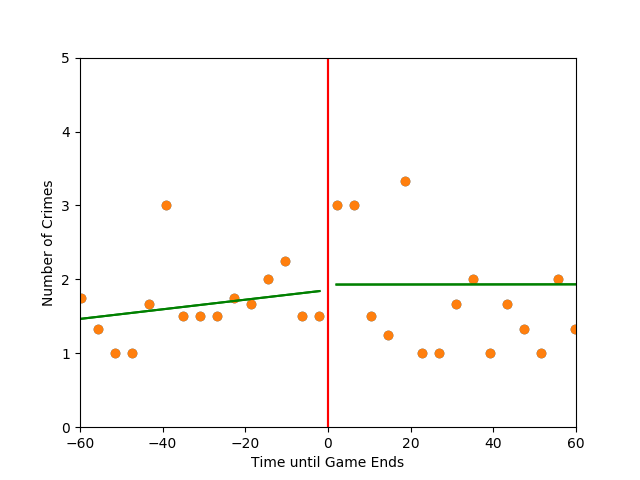
\includegraphics[scale = .65]{Linear2015}

\subsection*{Quadratic 2015}
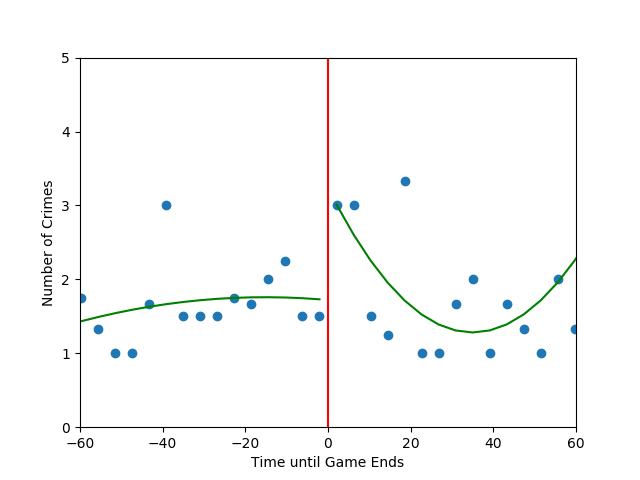
\includegraphics[scale = .65]{quad2015}

\section{Visual Evidence}
\subsection*{Linear 2016}
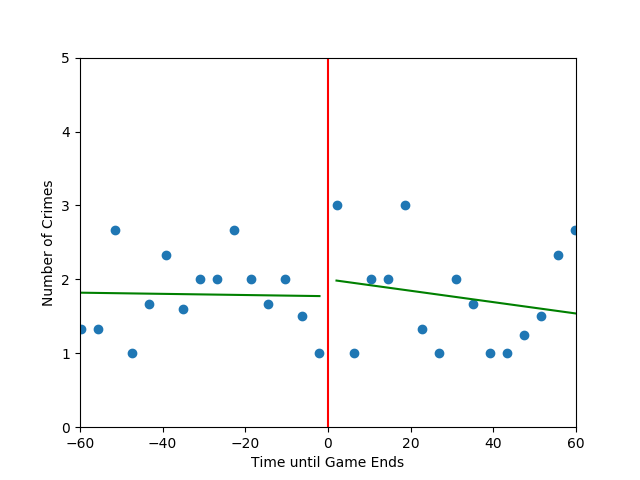
\includegraphics[scale = .65]{Linear2016}

\subsection*{Quadratic 2016}
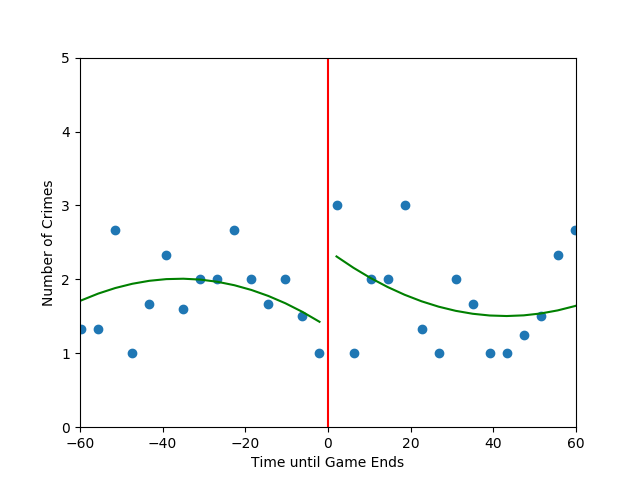
\includegraphics[scale = .65]{quad2016}
\newpage{}



\section*{Empirical Model}

I run 3 RDD specifications on each year of crime data:

\begin{equation}
C_t = \alpha + \beta Crowd + \gamma Time + \lambda Crowd * Time + \epsilon
\end{equation}

where $C_t$ the number of crimes that occur in a given 4 minute window near Washington Nationals Stadium. Crowd represents our treatment variable and indicates whether or not t is before or after the end of a baseball game. Time represents the number of minutes until or since that day's game ended.\\

This baseline model empirically tests the discontinuity (or lack thereof) of the linear fit plots above. The results from this estimation can be seen in Column 1 of Tables 1 and 2 below.

As expected from the visuals above, we do not observe a statistically significant discontinuity in either year using a linear fit specification.

\begin{equation}
C_t = \alpha + \beta Crowd + \gamma Time + \delta Time^2 +  \lambda Crowd * Time + \sigma Crowd * Time^2 + \epsilon
\end{equation}
 
Given the visual results recorded above, we know that using a quadratic fit not only fits the data better, but also illustrates more evidence of a discontinuity around the cut-point.  Therefore, the second specification fits a quadratic function, which is allowed to differ on either side of the cut-point.\\

The results from the estimation of equation 2 can be seen in column 2 of Tables 1 and 2 below. We note here that we do find a significant estimate in 2015 for our coefficient of interest, $\beta$. The 1.52 estimate, significant at the 5\% level, indicates that the crowds resulting from the baseball stadium may create about 1.5 extra crimes.

For the 2016 data, I also find a positive coefficient estimate, however, it is imprecisely estimated and indistinguishable from zero



\begin{equation}
C_t = \alpha + \beta Crowd + \gamma Time +  \lambda Crowd * Time + \sigma Crowd * Time^2 + \epsilon
\end{equation}
 
The third and final specification allows a quadratic fit on the right side of the cut-point and a linear fit on the left side. Results from this estimation can be found in column 3 of Tables 1 and 2 below. We do not find marked differences between these results and those from equation 2, a significant result in 2015, but not in 2016.\\
 
All told, these results suggest that the crowds emanating from Washington Nationals stadium may have an impact on criminal activity in the area, however, more evidence is required to establish a causal relationship. Further refinement of the empirical model is necessary. In particular, interactions on the games attendance must be added; here a game with high attendance and low attendance essentially apply the same treatment, according to our model. Data from more cities as and more years are also needed to establish a generalizable result.
\newpage
\section*{Table 1}
\begin{table}[hb!]
\begin{center}
\begin{tabular}{c|c|c|c|}
\toprule
 & \multicolumn{1}{c}{Model 1} & \multicolumn{1}{c}{Model 2} & \multicolumn{1}{c}{Model 3} \\
\midrule
(Intercept)   & $1.85^{***}$ & $1.72^{**}$ & $1.72^{**}$ \\
              & (0.37)     & (0.48)    & (0.48)    \\
Crowd         & 0.07       & $1.52^{*}$  & $1.52^{*}$  \\
              & (0.53)     & (0.68)    & (0.68)    \\
TimeBin       & 0.01       & -0.00     & -0.00     \\
              & (0.01)     & (0.03)    & (0.03)    \\
Crowd:TimeBin & -0.01      & $-0.11^{*}$ & $-0.11^{*}$ \\
              & (0.01)     & (0.04)    & (0.04)    \\
TimeSq        &            & -0.00     & -0.00     \\
              &            & (0.00)    & (0.00)    \\
Crowd:TimeSq  &            & $0.00^{**}$ & $0.00^{**}$ \\
              &            & (0.00)    & (0.00)    \\
\midrule
R$^2$         & 0.06       & 0.36      & 0.36      \\
Adj. R$^2$    & -0.04      & 0.25      & 0.25      \\
Num. obs.     & 34         & 34        & 34        \\
RMSE          & 0.77       & 0.65      & 0.65      \\
\bottomrule
\multicolumn{4}{l}{\scriptsize{$^{***}p<0.001$, $^{**}p<0.01$, $^*p<0.05$}}
\end{tabular}
\caption{RDD Model of 2015 Data}
\label{tab:3}
\end{center}
\end{table}
\newpage

\section*{Table 2}
\begin{table}[hb!]
\begin{center}
\begin{tabular}{c|c|c|c|}
\toprule
 & \multicolumn{1}{c}{Model 1} & \multicolumn{1}{c}{Model 2} & \multicolumn{1}{c}{Model 3} \\
\midrule
(Intercept)   & $1.77^{***}$ & $1.35^{**}$ & $1.35^{**}$ \\
              & (0.31)     & (0.46)    & (0.46)    \\
Crowd         & 0.23       & 1.04      & 1.04      \\
              & (0.43)     & (0.64)    & (0.64)    \\
TimeBin       & -0.00      & -0.04     & -0.04     \\
              & (0.01)     & (0.03)    & (0.03)    \\
Crowd:TimeBin & -0.01      & -0.00     & -0.00     \\
              & (0.01)     & (0.04)    & (0.04)    \\
TimeSq        &            & -0.00     & -0.00     \\
              &            & (0.00)    & (0.00)    \\
Crowd:TimeSq  &            & 0.00      & 0.00      \\
              &            & (0.00)    & (0.00)    \\
\midrule
R$^2$         & 0.04       & 0.13      & 0.13      \\
Adj. R$^2$    & -0.06      & -0.03     & -0.03     \\
Num. obs.     & 34         & 34        & 34        \\
RMSE          & 0.63       & 0.62      & 0.62      \\
\bottomrule
\multicolumn{4}{l}{\scriptsize{$^{***}p<0.001$, $^{**}p<0.01$, $^*p<0.05$}}
\end{tabular}
\caption{RDD Model of 2016 Data}
\label{tab:3}
\end{center}
\end{table}


\end{document}